%!TEX root = ../thesis.tex
%*******************************************************************************
%*********************************** First Chapter *****************************
%*******************************************************************************

\chapter{Introduction}  %Title of the First Chapter
\label{Introduction}

\ifpdf
    \graphicspath{{Chapter1/Figs/Raster/}{Chapter1/Figs/PDF/}{Chapter1/Figs/}}
\else
    \graphicspath{{Chapter1/Figs/Vector/}{Chapter1/Figs/}}
\fi
\section{Background}
Climate change has been a well-known problem among scientists for a long time. The first paper warning about the effects of the increment of carbon dioxide in the atmosphere is from 1976 \cite{manabe_thermal_1967}, while in a study of 1976 \cite{keeling_atmospheric_1976} it was observed for the first time. In 1988, the World Meteorological Organization Established the Intergovernmental Panel On Climate Change (IPCC) \cite{baker_1989}, which is the leading organization evaluating climate change up to date. As shown in \cite{santos_climate_2021}, the researchers' interest in climate change grew significantly after 1990. 

\begin{figure}[H]
    \centering
    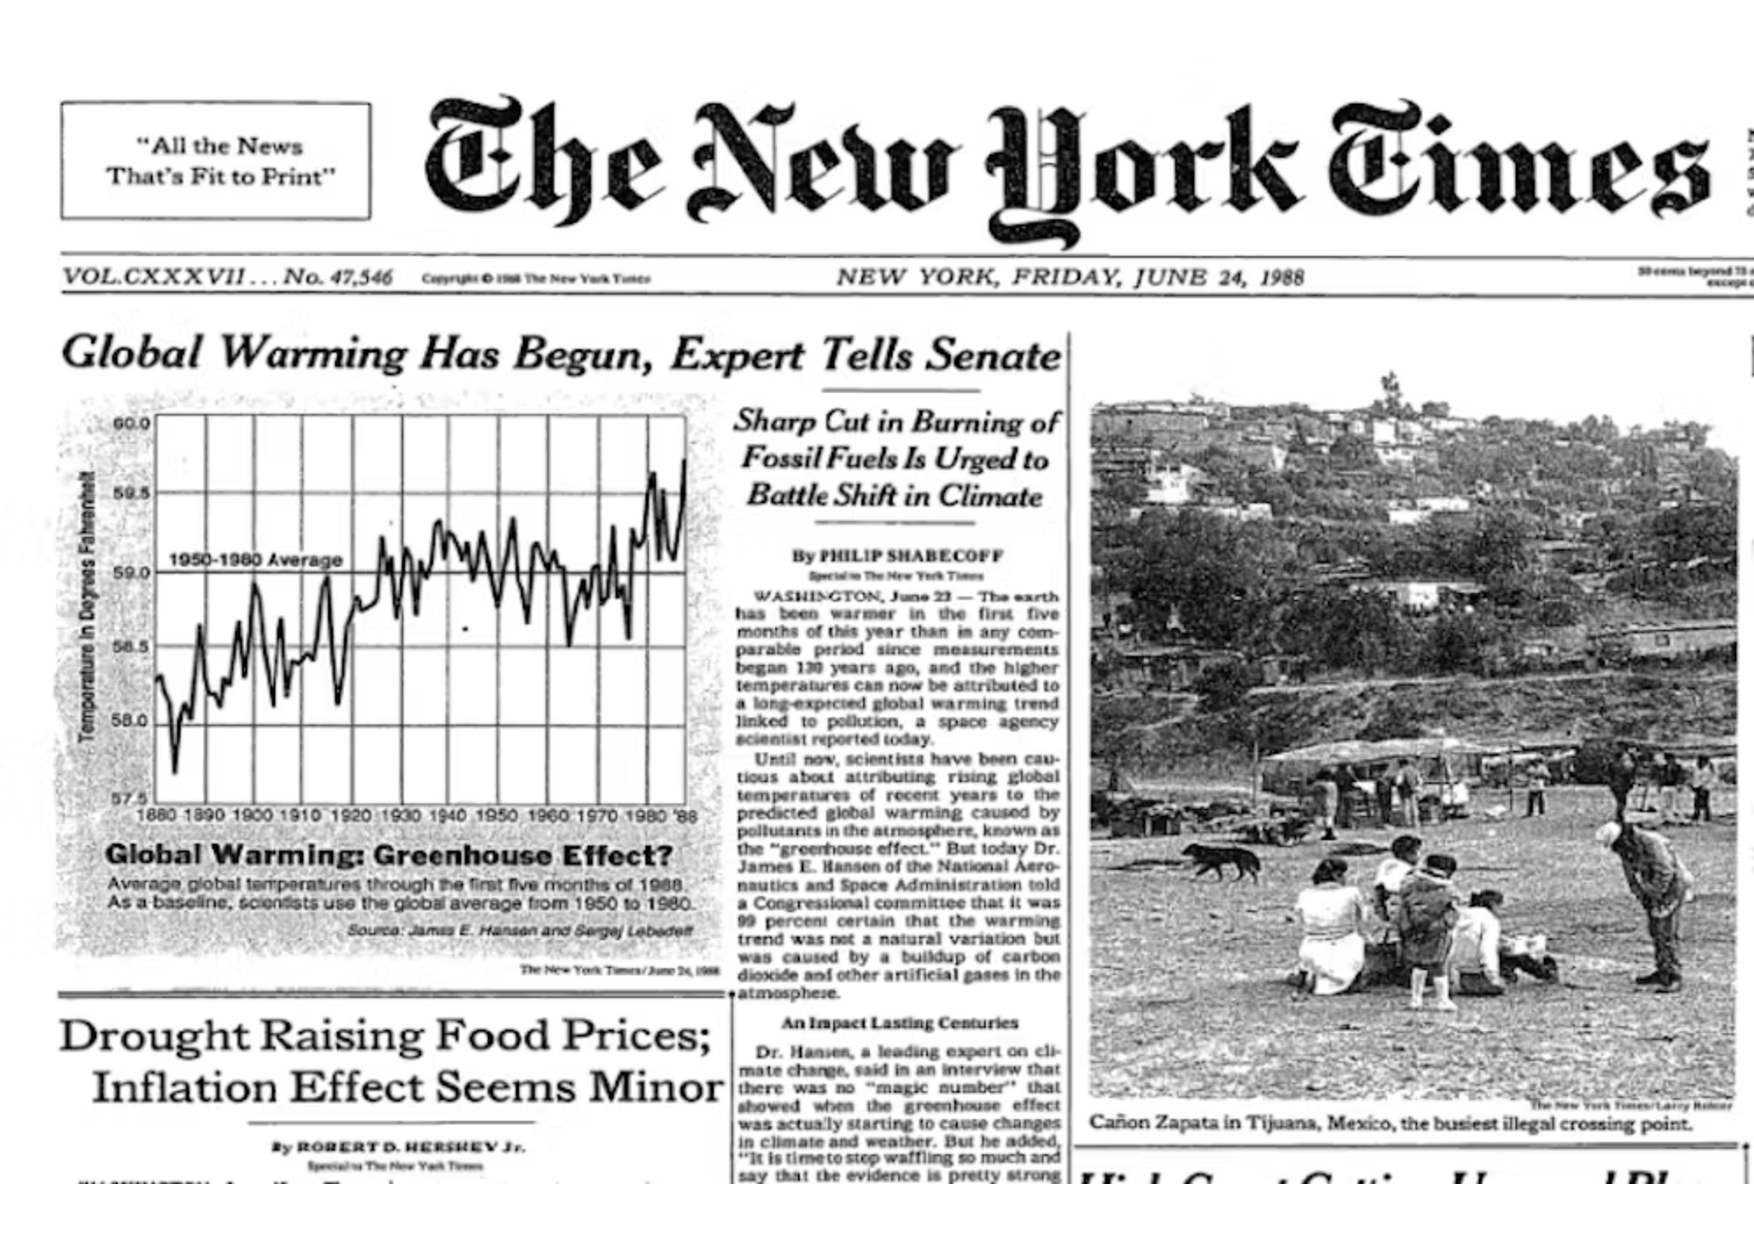
\includegraphics[width=0.75\linewidth]{Chapter1/figures/global_warming copy.pdf}
    \caption{Front page of NY Times, June 24, 1988 }
    \label{fig:enter-label}
\end{figure}

The issue has become mainstream only in the past few years since, partially due to Greta Thunberg \cite{sabherwal_greta_2021} and Fridays for Future, people grew more aware of the problem. As we can see in Fig \ref{fig:google_greta}, only after 2019 people started searching for, and talk about, a 'climate crisis' \footnote{we choose this term because it is not descriptive as climate change but focus on the negative version of it}, underlining the urgency with which we should act. It is also true that the strikes caused inconvenience to many ordinary citizens trying to reach their workplaces. As a consequence someone may have developed some hostility toward this activism and, thus, toward climate change. In fact, an increase in polarization has been detected after the strikes \cite{Falkenberg_climate_2022}.
\\

\begin{figure}
    \centering
    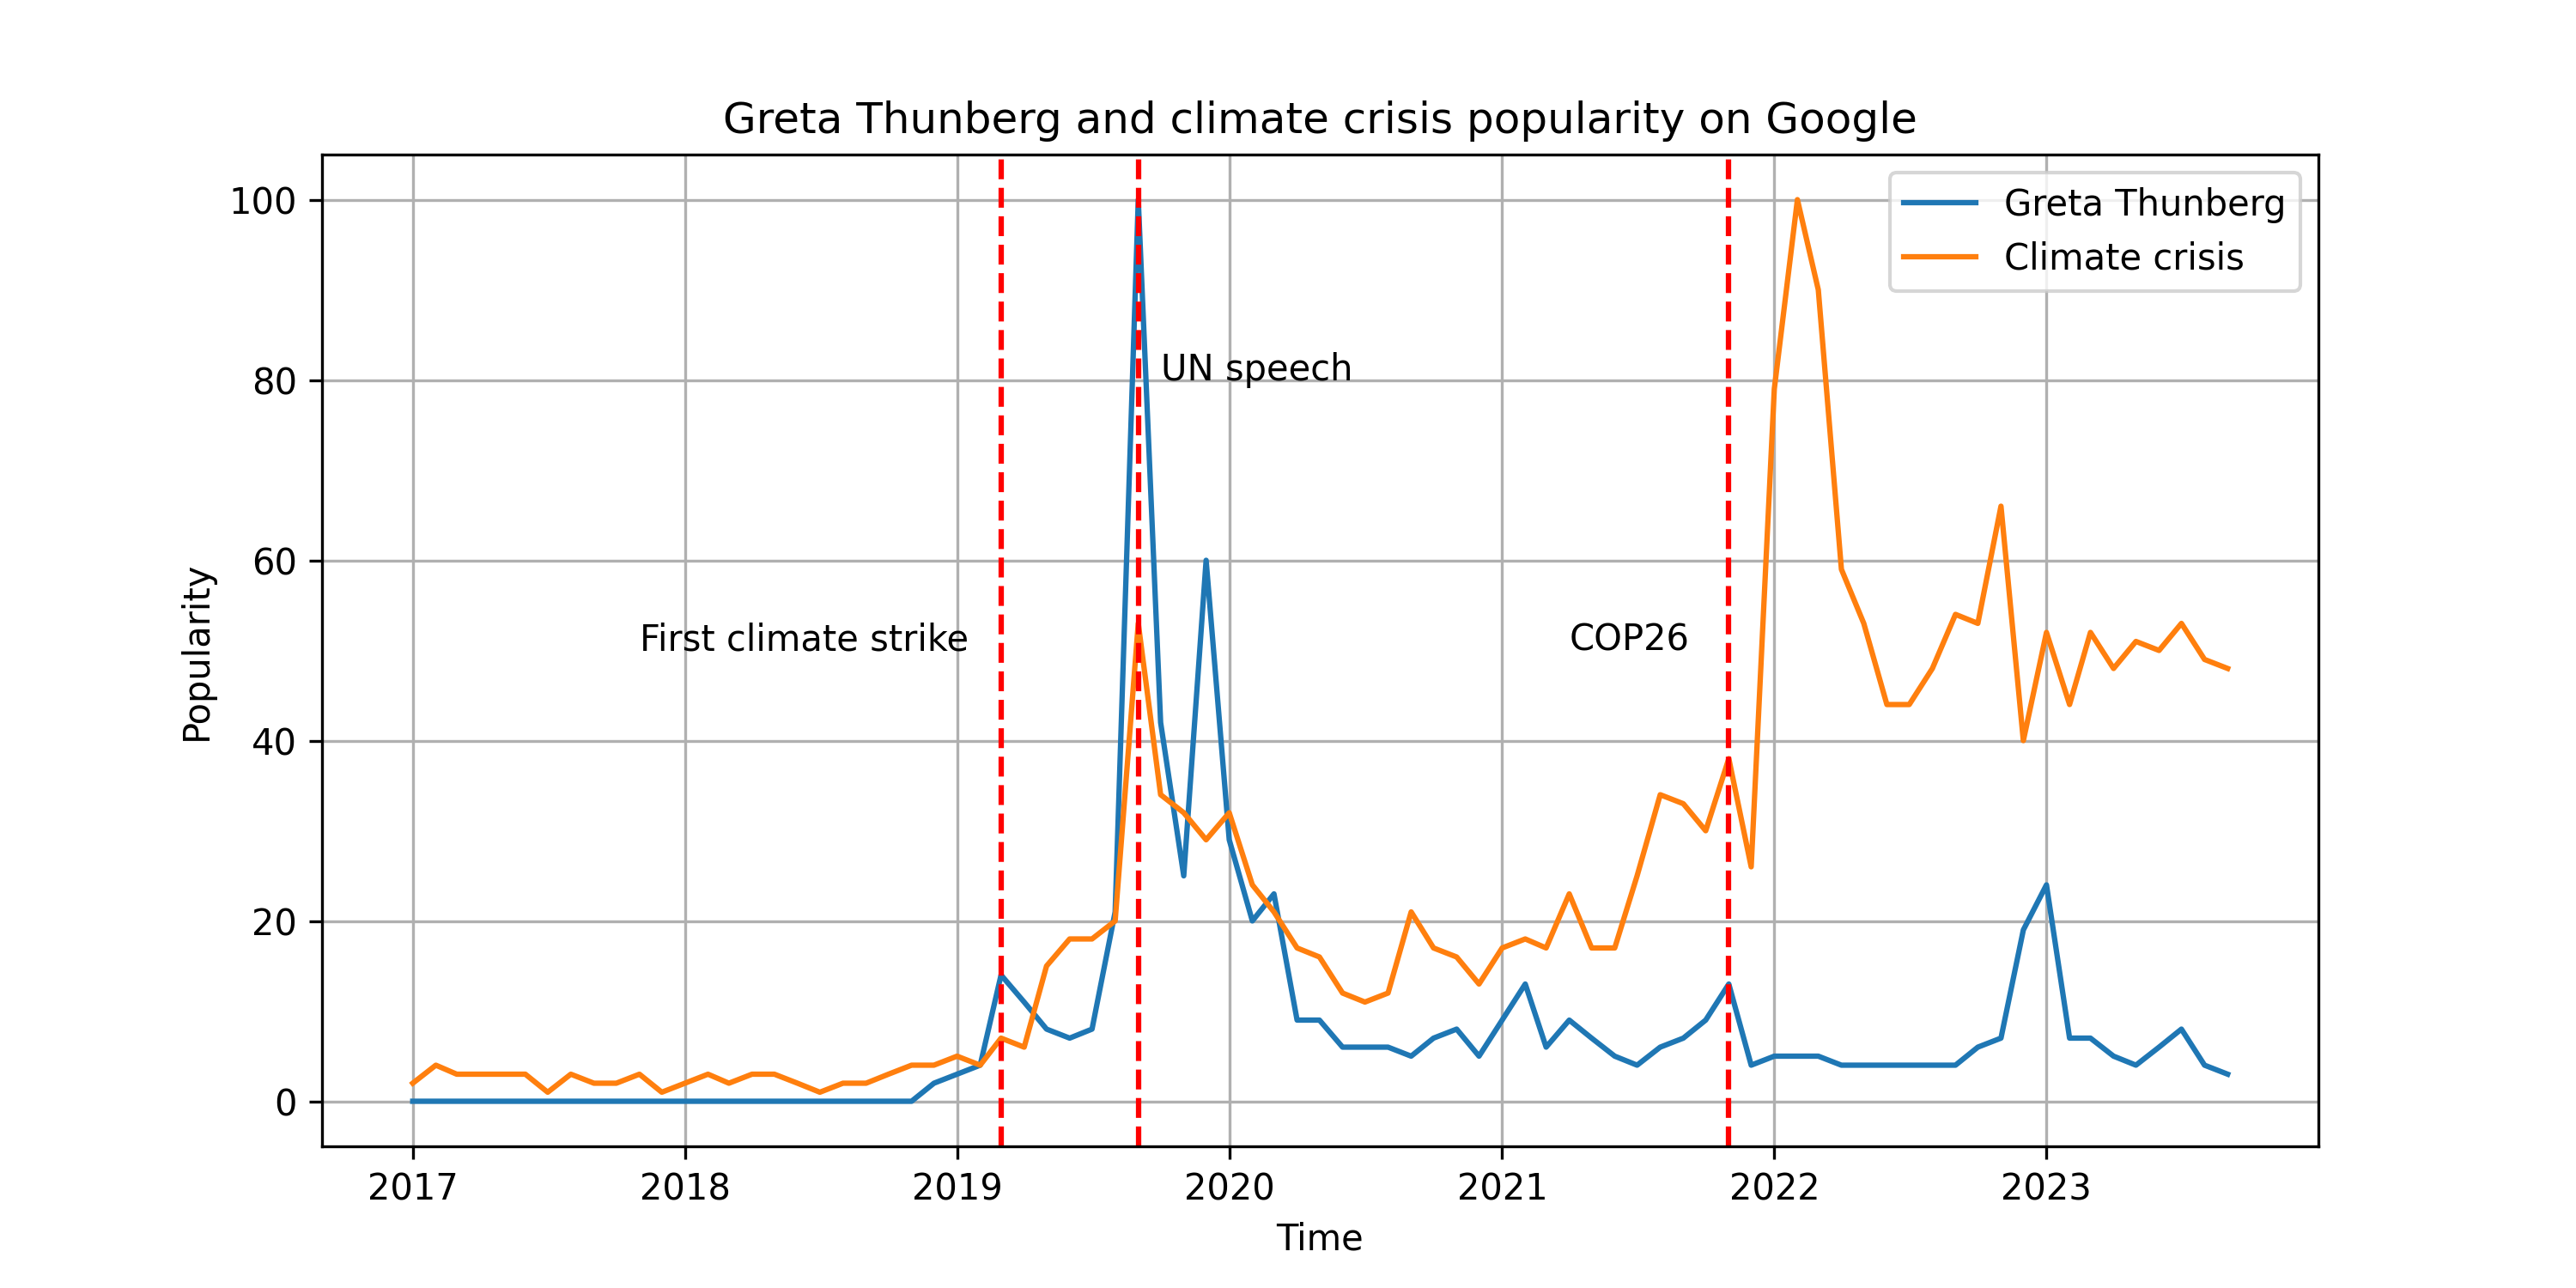
\includegraphics[width=0.85\linewidth]{Chapter1/figures/greta_climate_crisis.png}
    \caption{interest on Google over the time of Greta Thunberg and climate crisis}
    \label{fig:google_greta}
\end{figure}

Conferences of Parties (COP) are conferences where the highest political figures of many countries meet and talk about climate emergencies. This serves also to bring the discussion to the masses, increasing awareness on the problem.
In particular, Twitter is a place where part of the political debate takes place \cite{Pew_twitter_2022} and political events like this can be studied thanks to the availability of big amount of data.


The increasing polarization poses a significant challenge to the mitigation of the harmful impacts of climate change; for this reason, understanding the root cause has the potential to speed up the reduction of emissions, not having to deal with strong opponents. This can have the effect to save human lives and resources.



\paragraph{Conference of Parties}
Conferences of Parties are yearly conferences organized by the United Nations where the topic of discussion is climate change; the first was held in 1995 in Berlin, and the ones that ended with a document to ratify are:
\begin{itemize}
    \item \textbf{COP3}: Kyoto Protocol (1997) It was the first treaty to mandate countries to cut greenhouse gas emissions that was legally binding, but this was true only for developed countries, therefore exluding China and India.
    \item \textbf{COP21}: The Paris Agreement (2015) is a global accord that aims at limiting global warming to well below 2 degrees Celsius (preferably to 1.5 degrees Celsius) compared to pre-industrial levels by requiring all countries to set their own emissions reduction targets. It is considered more effective and inclusive than the Kyoto Protocol because it involves all countries, allows for flexibility in setting emissions targets, and includes a robust system for transparency and accountability.
    \item \textbf{COP26}: Glasgow Climate Pact (2021) is a crucial agreement in the global effort to combat climate change. It is the direct consequence and a refinement of the Paris agreement. It includes significant commitments to address the urgent challenges of climate change, such as phasing down coal usage, increasing climate finance for adaptation, strengthening international cooperation, and supporting countries which are transitioning to low-carbon economies. However, not everyone agrees with the outcomes of the conference: for example, \cite{arora_cop26_2021} shows how the previous goal has not been 
 achieved and how the roadmap is not clear. While \cite{layna_promises_2022} underlines how the politics decisions are not based on the IPCC report, which is the most trusted scientific reference for climate change. 

\end{itemize}


\\
The focus of this work will be on COP26 which is the one that occurred in a context of popular agitation toward the topic. Additionally, a spike in the climate crisis interest has been detected right after it. Then, a comparison between COP21 and COP26 will be done due to its analogies, in fact the Glasgow climate pact exists as a more specific definition of the too general Paris agreement. Both happen in a context of political constrast, during 2017,  president Trump of  the United States  decided to withdraw from the Paris agreement because it would have undermined the US economy. This caused disappoinement to all the others members, especially the developing countries which are the most affected by global warming effects.
\\

This work lays its foundations on the research of Falkenberg et al. \cite{falkenberg_growing_2022}, who discovered that COP26 was way more polarized than COP21. Using a similar approach, the ideological polarization will be explored topic by topic using cutting edge technologies such as transformers and by exploiting the complexity of multilayer networks. 

There is not a universally agreed definition of polarization. Ref \cite{madgalena_polarization} help disambiguate the various definitions that fall under the term polarization. It distinguish between sociopolitical, group and individual polarization. Our focus will be on the sociopolitical one which concern the polarization of the influential individuals within the parties,  called elite polarization, which is defined  as the alignment of the political leader with all the positions of its own party. There is a general agreement between social and political scientist that elites are polarized, while it is unclear  if the masses are also polarized in the same way, since the results can depend on the methodology.



In this paper, we will operationalize it using what stated in \cite{bramson_understanding_2017}, the same used by Falkenberg, which is: "The most common measure of polarization in the political literature is probably bimodality, which is the idea that the population can be usefully broken down into two subpopulations". 
In the case at hand, the two sub-populations are pro-climate and climate skeptics.



\section{Research Questions}
Due to the structure of this research, we can now answer a new set of questions related to intra-topic polarization. The first two look at the networks at a macro level focusing on the topology. The most straightforward is the first, RQ1, which aims at inspecting the topics that are driving the polarization of the entire COP26. Secondly, RQ2 wants to identify whether these topics have always been polarized compared to COP21.

Then, we the focus will shift to a micro level with some questions related to the users, similarly to 
\cite{garimella2017longterm} that  investigated the users retweet from both sides, but in addition we are interested also in the presence in multiple topics.

In particular, RQ3 looks into whether  users are polarized in the same way over the different topics or if there are topics in which they are on the opposite side of the spectrum. RQ4 instead investigates whether the most active users, both in term of number of tweets and the presence on multiple topics, are more polarized than the others.

Summarizing, the questions are:

\begin{enumerate}
    \item  Which are the most polarizing topics discussed on Twitter during Cop 26?
    \item How did topics evolve between cop21 and cop26?
    \item Is the single-user polarization different across different topics? 
    \item Does the polarization of users differ depending on whether the users are present in multiple topics rather than just one?


\end{enumerate}

\section{Structure}
This thesis is structured to provide a comprehensive exploration of  topic modeling applied unstructured text organized in a multilayer network. It is divided into a series of chapters, each serving a distinct purpose in advancing the understanding of the subject matter. 

Chapter \ref{Ch:related} touches the state of the art of all the matters used in this work, first exploring the most recent topic modeling techniques with the goal to select the best suited to our scenario; second, a comprehensive review of networks, in particular social networks and multilayer networks, and how polarization is computed.

Chapter \ref{ch:data} presents the dataset along with some statistics about it.

Chapter \ref{ch:methodology} is the core of this work, the first section covers the evaluation of several topic modeling techniques, using two approaches, unsupervised and supervised, several models have been tested from traditional to the ones based on neural networks. After identifying the best performing model, the network section shows the pipeline that allows to build a multilayer network based on the topics starting from the raw tweets. Finally for each layer it is computed a polarization score using the latent ideology score given to the users.

Chapter \ref{ch:res}  show the answer to the research question posed above.  

Chapter \ref{ch:conclusion} wrap up everything and show some other research that can be done using the same methodology.






%********************************** %First Section  **************************************

\nomenclature[z-DEM]{DEM}{Discrete Element Method}
